%
% LaTeX2e template for FIT2002
%


\documentclass[a4j,twocolumn]{ujarticle}
\usepackage[dvipdfmx]{graphicx}
\usepackage[dvipdfmx]{color}
\usepackage{ascmac}
\usepackage{url}



\makeatletter
\def\section{\@startsection{section}{1}{\z@}{2ex plus .2ex minus .2ex}%
{.5ex plus .2ex minus .2ex}{\large\bfseries}}
\def\thesection{\arabic{section}.}
\def\subsection{\@startsection{subsection}{1}{\z@}{.7ex plus .2ex minus .2ex}%
{.5ex plus .2ex minus .2ex}{\normalsize\bfseries}}
\def\thesubsection{\arabic{section}.\arabic{subsection}}
\def\thefootnote{\fnsymbol{footnote}}
\makeatother


\def\baselinestretch{0.8}

\setlength{\textheight}{23.5cm}%297-30-27 - 5
\setlength{\textwidth}{17.4cm}%210-18-18 - 10
%\setlength{\headheight}{0.0in}
\setlength{\headsep}{0.0in}
\setlength{\oddsidemargin}{-.9cm}%+3
\setlength{\evensidemargin}{-.9cm}%+3
\setlength{\columnsep}{7mm}


% local settings

% end of local settings


\begin{document}
    \pagestyle{empty}
    \thispagestyle{empty}

    \twocolumn[%
        \begin{center}
        {\Large 今学期作ったもの}
            \vspace{.5ex}

            {\Large\sffamily }\vspace{1ex}



            \large
            \mbox{}
            \hfil
            \setcounter{footnote}{2}
            {\bfseries Sociable Robots B1 澤田 開杜(sabaniki)}${}^\thefootnote$
            \hfil
            \setcounter{footnote}{3}
            \hfil
            \mbox{}

            \mbox{}
            \hfil
            {\sffamily}
            \hfil
            {\sffamily}
            \hfil
            \mbox{}
            \hfil

        \end{center}
    ]

    \setcounter{footnote}{2}
    \footnotetext{慶應義塾大学 環境情報学部}

\section{概要}
私が今学期製作した4つのプロダクトについて報告する。4つのプロダクトとは以下の表\ref{ProductsSem}に示した通りである。
毎月別のプロダクトに着手し、そのうち2つについては現在も開発を積極的に続けている。

\begin{table}[h]
    \caption{今学期製作したもの一覧}
    \label{ProductsSem}
    \centering
    \begin{tabular}{lcr}
        \hline
        着手時期 & 名前 \\
        \hline \hline
        4月 & ARplusR \\
        5月 & MTG-Shuffle \\
        6月〜 & IoT-Fam \\
        7月〜 & Over-Comment \\
        \hline
    \end{tabular}
\end{table}

\section{ARplusR}
\subsection{概要}
プロダクトの名前のARplusRとはAR+Robotを意味している。ARとロボットの組み合わせに興味が湧いたため、
プロトタイプとして、ARの入門も兼ねて作成したものである。
今回は実物のロボットを使わずに、ロボットも仮のものをAR上のオブジェクトで作成した。

\subsection{実装した機能}
以下に図\ref{ARRobotImage}として実際のアプリケーションのスクリーンショットを示す。
平面をアプリケーション上で検知し、その面に対して障害物に見立てた灰色の立方体を設置することができる。
すると、ロボットに見立てた黄色の立方体がその障害物を避けて前進するというものである。

\begin{figure}[h]
\centering
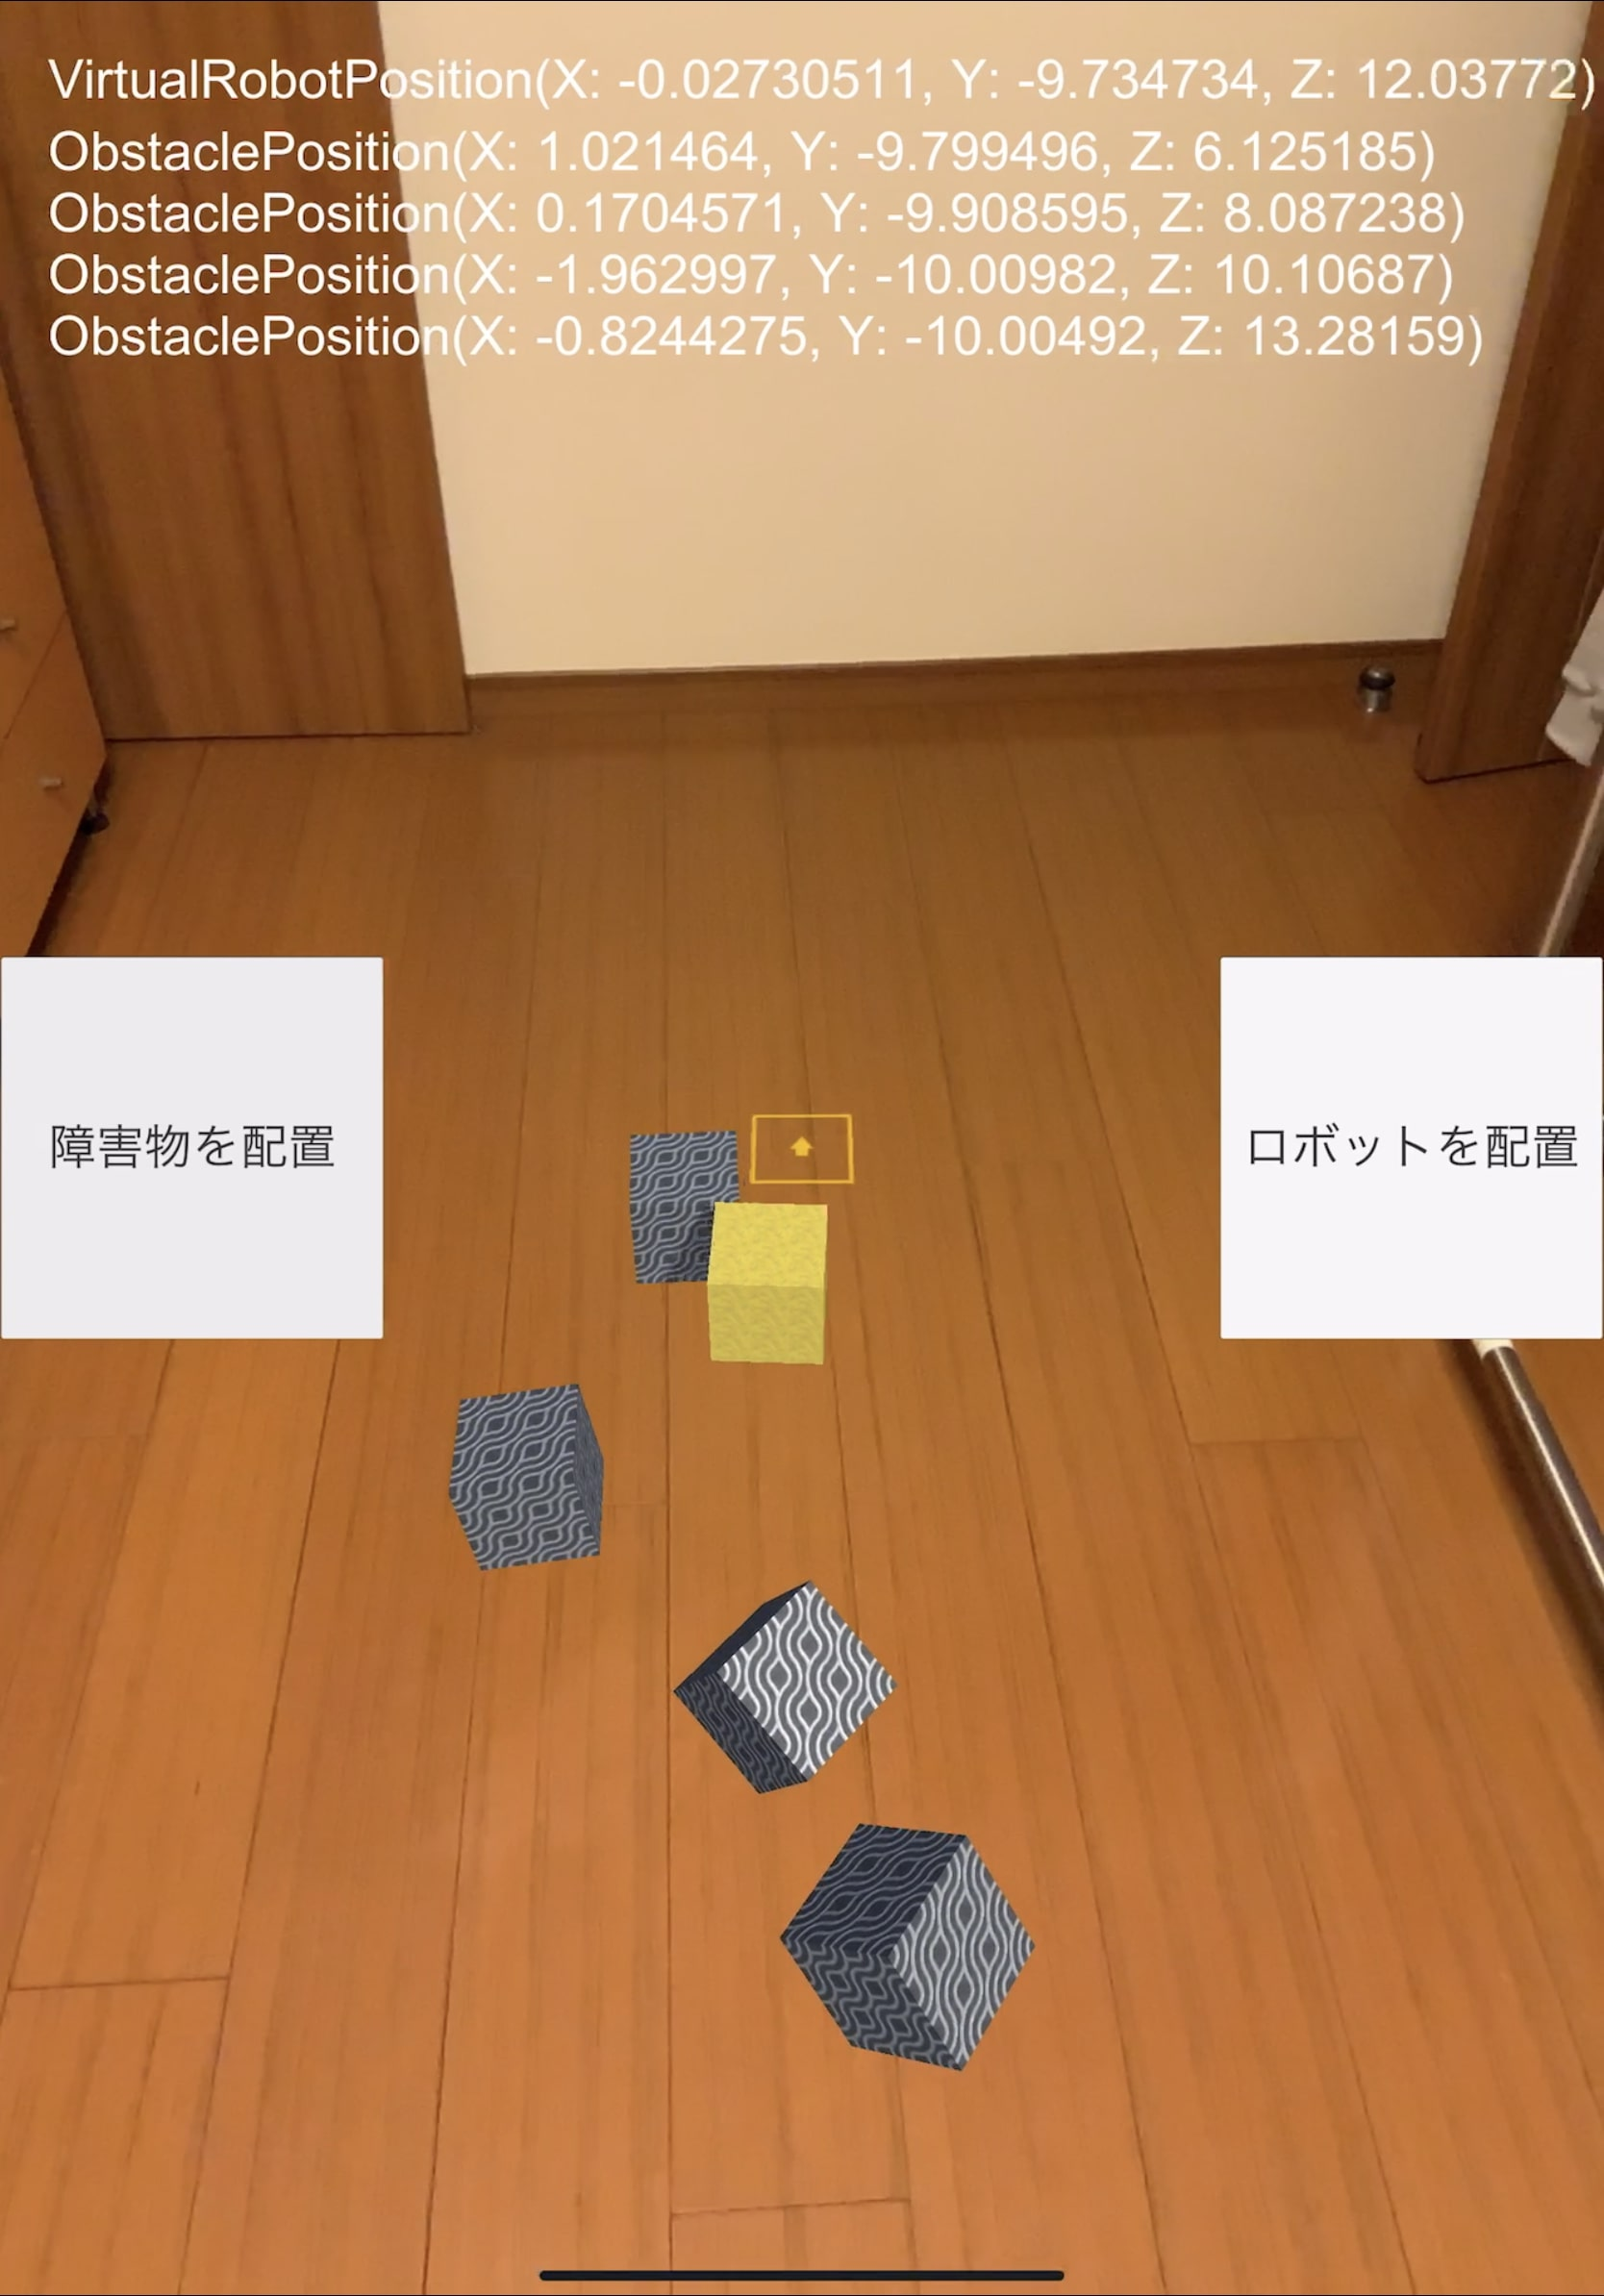
\includegraphics[width=4cm]{../assets/AR-Robot.jpg}
\caption{実際に作ったARアプリ}
\label{ARRobotImage}
\end{figure}

\subsection{展望}
今回は元々「ARを使うことで人間は視覚的にロボットに対して仮想的な情報を与えられる」
という部分に興味を持って取り組んだものだったが、
その特性を用いて具体的なプロトタイプを製作することはできなかった。
ロボットの進行方向をAR上で指示したり逆にロボットに侵入されたくない場所を指定するなどの案は出たが、
実現することはできなかった。
ARに興味がなくなったわけではなく、Apple Glassなどのまだ見ぬ新しいデバイスにも興味があるため、
今後も発展させていきたい。

\section{MTG-Shuffle}
\subsection{概要}
弊研究会では毎週火曜日に進捗報告とその週の目標を決めるグループ別のミーティングが行われる。
そのグループは院生をリーダとしてそこに均等になるように学部生が分かれるという形式であるが、
毎週のグループ分けが面倒であるという点があった。その問題を解決するべく、新人課題として取り組んだ。

\subsection{実装した機能}
以下に図\ref{MtgShuffleImage}としてアプリケーションのスクリーンショットを示す。
この図の通り、ランダムにグループを分ける機能を実装し、それを閲覧可能にしている。
また、ランダムにグループを分けるアルゴリズムは
院生や学部生の数が変化に依存しない仕組みになっている。
グループのリセットは一日に一度、誰か一人が行うことができる。
リセット限度を一日一度にしているため、
複数人がグループをリセットしてしまうことによる混乱が生じないよう工夫している。

\begin{figure}[h]
\centering
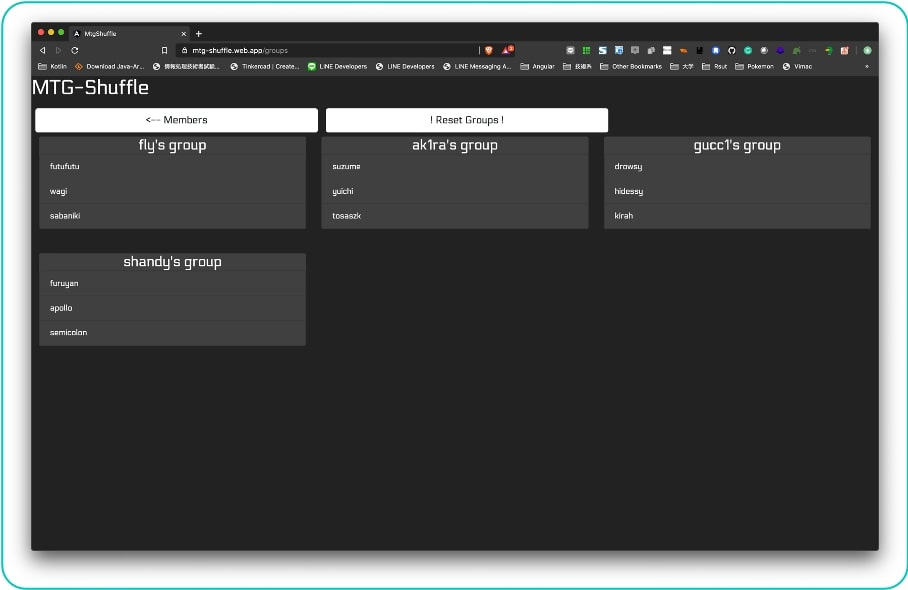
\includegraphics[width=4cm]{../assets/MTG-Shuffle.jpg}
\caption{MTG-Shuffle}
\label{MtgShuffleImage}
\end{figure}

\subsection{展望}
人数に依存しないアルゴリズムを考案するよりも前に
欠席者を除外してグループを作成する機能をつけるべきであったが、それがまだ実装されていない。
また、メンバーのCRUD機能も実装されておらず、いずれも仮のボタンが設置されているだけなので
なるべく早く実装する必要がある。また、完全にランダムにすると同じ人と当たりやすく感じることが
わかったため、同じ人と連続で当たりにくくなるようなアルゴリズムを考案し、実装する必要もある。

\section{IoT-Fam}
\subsection{概要}
最終的な完成形としては以下に図\ref{IoTFam}として示した通りである。
図ではSlackを使用しているが、家族LINEにIoTが参加し、
そこでのIoT同士の会話の中に人間が参加するというものである。
今現在のAlexaやGoogleHomeなどの中心的な存在があり、そこに対して人間が指示を出すと
各IoTが受動的で無機質にタスクをこなすという状態に対して私は疑問を感じたため製作を始めた。

\begin{figure}[h]
\centering
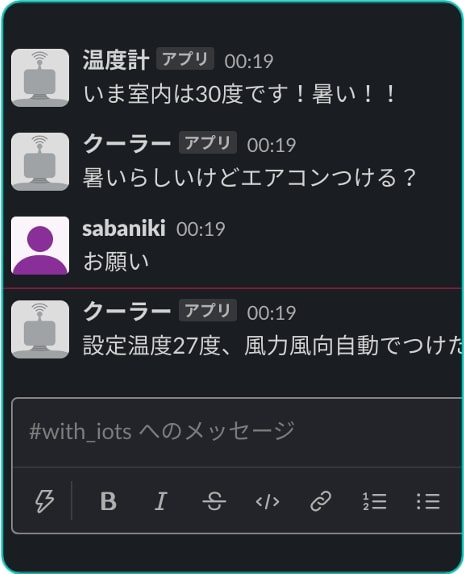
\includegraphics[width=4cm]{../assets/IoT-Fam.jpg}
\caption{IoT-Fam}
\label{IoTFam}
\end{figure}

\section{Over-Comment}
Over-Commentについてお話します

\bibliographystyle{junsrt}
\bibliography{bib.bib}



\end{document}
